\documentclass{article}
\usepackage[utf8]{inputenc}
\usepackage[spanish]{babel}
\usepackage{graphicx}
\usepackage{float}

\title{Práctica 3. Segunda Parte: Servidor Replicado}
\author{Noelia Escalera Mejías}

\begin{document}
	\maketitle
	\section{Método de comunicación}
	Para que las dos réplicas cooperen entre sí, se ha creado un método buscar réplica, que devolverá la otra réplica o null si no la encuentra. Se llamará a este método cada vez que nos queramos comunicar con otra réplica.
	\section{Funcionamiento del cliente}
	\begin{enumerate}
		\item Lo primero que haremos en el cliente será buscar una réplica del servidor (se ha elegido la réplica 1 por defecto).
		\begin{figure}[H]
			\centering
			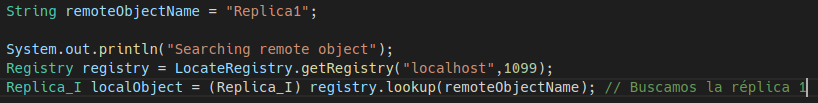
\includegraphics[totalheight=1.55cm]{img/1.png}
		\end{figure}
		\item Preguntamos al cliente si quiere registrarse o iniciar sesión
		\begin{figure}[H]
			\centering
			
\includegraphics[totalheight=1.5cm]{img/2.png}
		\end{figure}
		\item Si el cliente elige registrarse, pediremos un nombre de usuario (no puede estar ya escogido) y una contraseña.
		\begin{figure}[H]
			\centering
			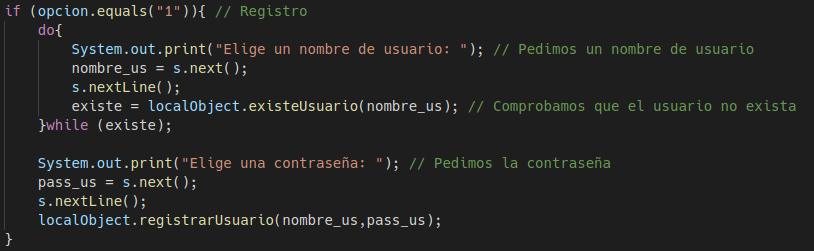
\includegraphics[totalheight=3.85cm]{img/3.png}
		\end{figure}
		\item Si el usuario elige inicio de sesión, se le pedirán los credenciales y no se le dejará entrar hasta que sean correctos.
		\begin{figure}[H]
			\centering
			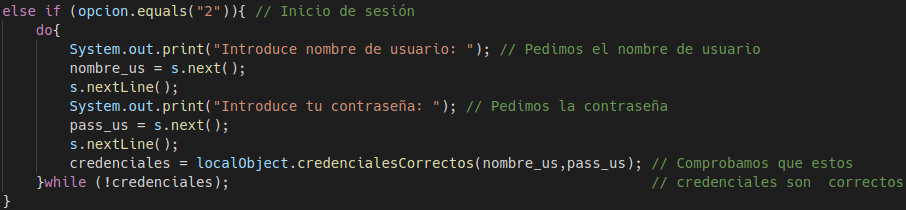
\includegraphics[totalheight=3cm]{img/4.png}
		\end{figure}
		\item Una vez hecho este paso, comprobaremos la réplica en la que está registrada el usuario y a partir de ahora haremos todas las consultas a ella.
		 \begin{figure}[H]
		 	\centering
		 	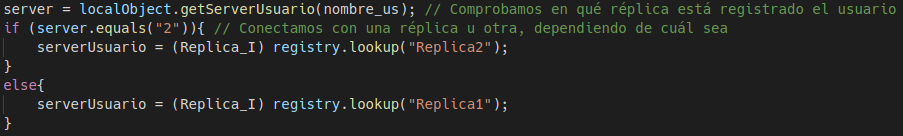
\includegraphics[totalheight=1.91cm]{img/5.png}
		 \end{figure}
	 	\item Luego preguntaremos qué acción se quiere realizar, esto se repetirá hasta que el usuario quiera salir
	 	\begin{figure}[H]
	 		\centering
	 		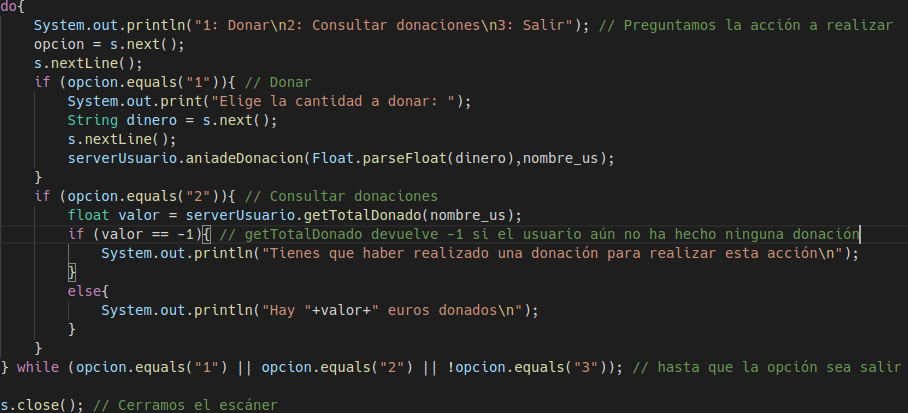
\includegraphics[totalheight=5.7cm]{img/6.png}
	 	\end{figure}
	\end{enumerate}
	\section{Explicación de los métodos del servidor}
	Estos son los métodos implementados en el servidor:
	\begin{figure}[H]
		\centering
		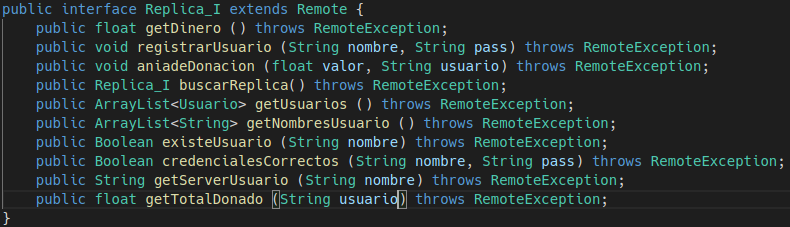
\includegraphics[totalheight=3.5cm]{img/7.png}
	\end{figure}
	Se pondrá de ejemplo la implementación en la réplica 1, la implementación en la réplica 2 es similar
	\begin{enumerate}
		\item {\bf getDinero.} Devuelve el dinero donado en esa réplica.
		\begin{figure}[H]
			\centering
			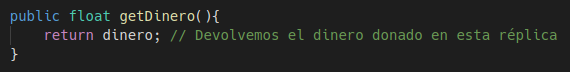
\includegraphics[totalheight=1.55cm]{img/8.png}
		\end{figure}
		\item {\bf registrarUsuario.}  Registramos un usuario en el sistema.
		\begin{figure}[H]
			\centering
			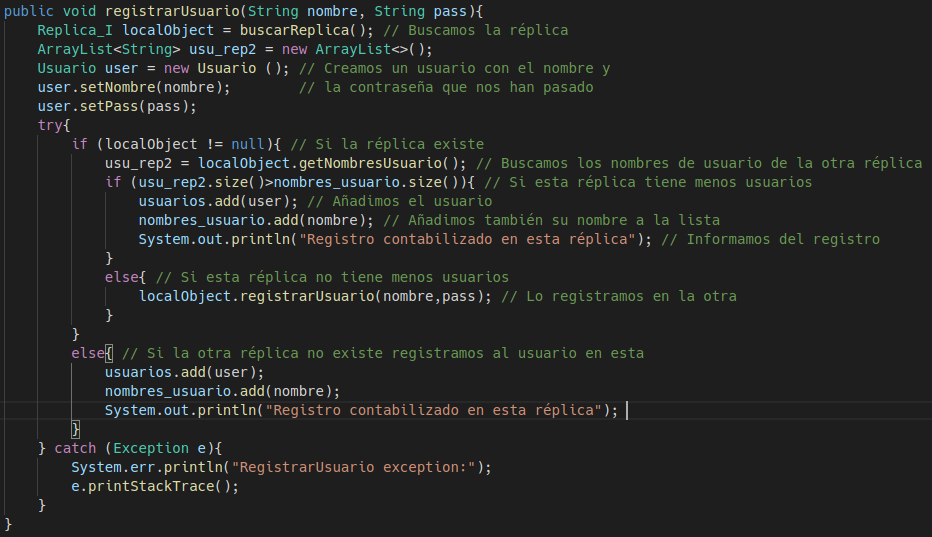
\includegraphics[totalheight=7cm]{img/9.png}
			\end{figure}
		\item {\bf aniadeDonacion.} Un usuario dona al servidor.
		\begin{figure}[H]
			\centering
			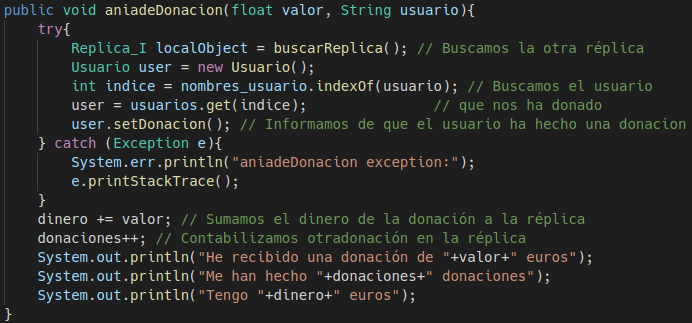
\includegraphics[totalheight=5.5cm]{img/10.png}
		\end{figure}
		\item {\bf buscarReplica.} Buscamos la otra réplica.
		\begin{figure}[H]
			\centering
			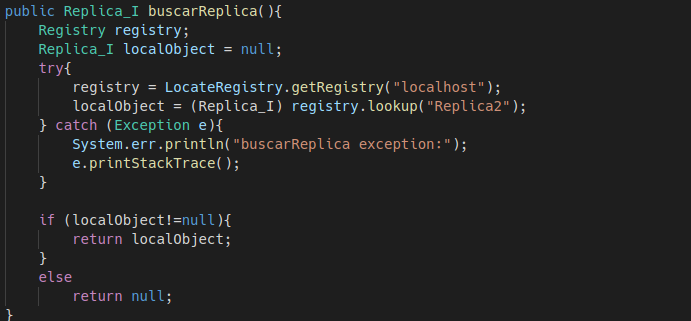
\includegraphics[totalheight=6cm]{img/11.png}
		\end{figure}
		\item {\bf getUsuarios.} Consultamos la lista de entidades usuario de una réplica.
		\begin{figure}[H]
			\centering
			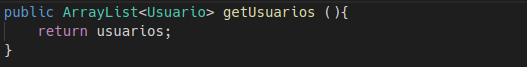
\includegraphics[totalheight=1.65cm]{img/12.png}
		\end{figure}
		\item {\bf getNombresUsuario.} Consultamos la lista de nombres de usuario de una réplica.
		\begin{figure}[H]
			\centering
			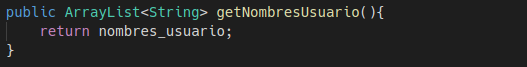
\includegraphics[totalheight=1.65cm]{img/13.png}
		\end{figure}
		\item {\bf existeUsuario.} Comprobamos si un usuario existe.
		\begin{figure}[H]
			\centering
			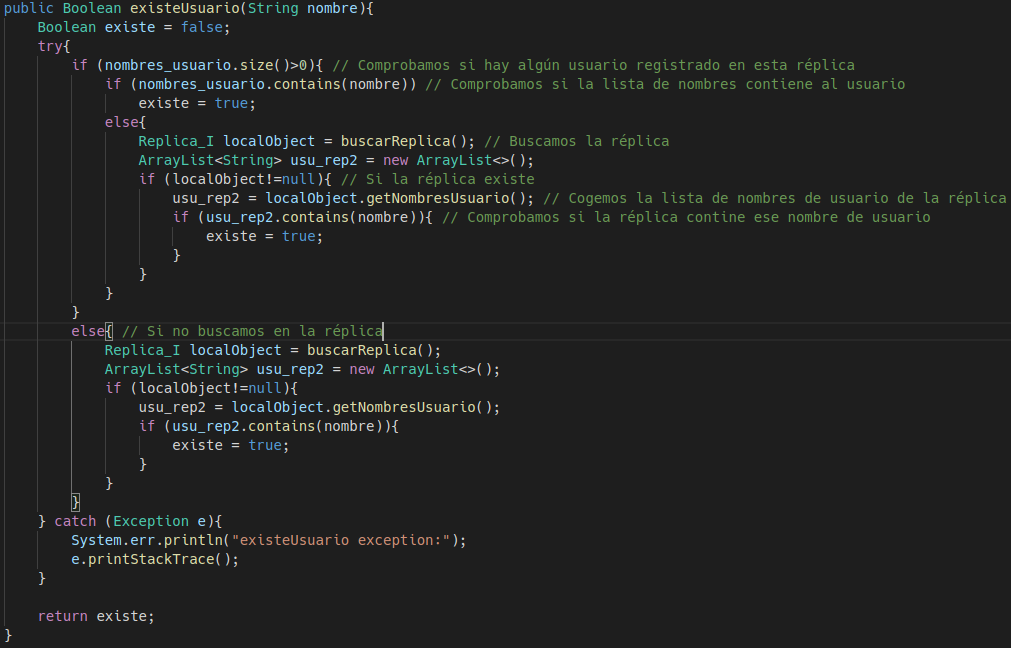
\includegraphics[totalheight=8cm]{img/14.png}
		\end{figure}
		\item {\bf credencialesCorrectos.} Comprueba si los credenciales introducidos al iniciar sesión son correctos.
		\begin{figure}[H]
			\centering
			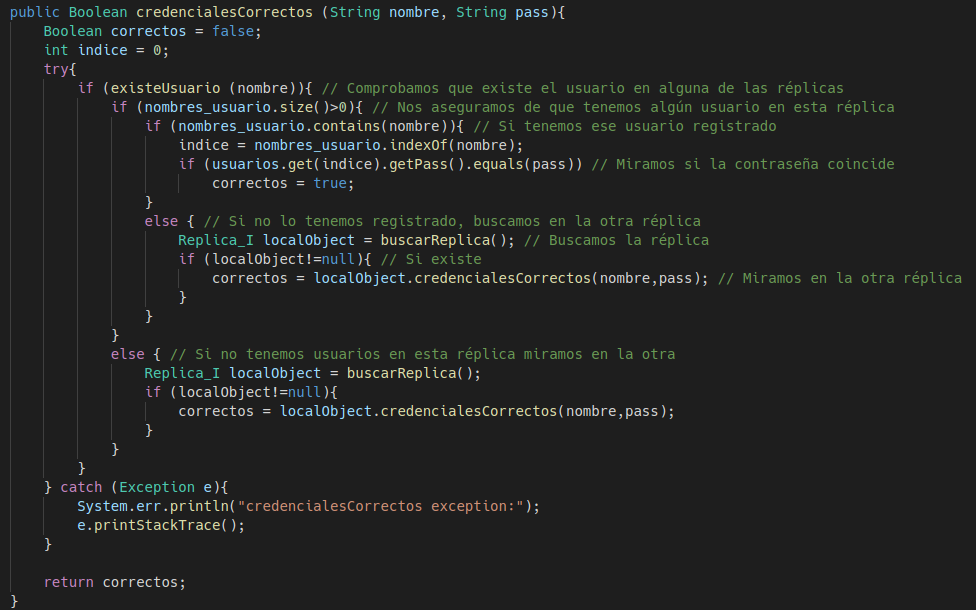
\includegraphics[totalheight=7.8cm]{img/15.png}
		\end{figure}
		\item {\bf getServerUsuario.} Comprobamos en qué réplica está registrado un usuario.
		\begin{figure}[H]
			\centering
			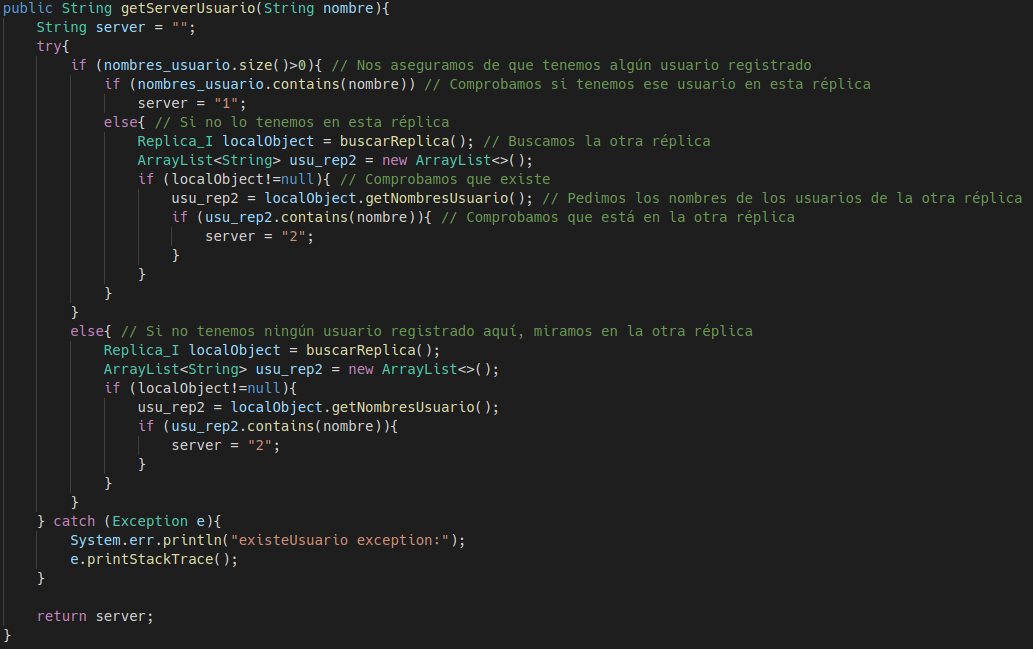
\includegraphics[totalheight=8cm]{img/16.png}
		\end{figure}
		\item {\bf getTotalDonado.} Comprobamos el total de dinero donado a las 2 réplicas.
		\begin{figure}[H]
			\centering
			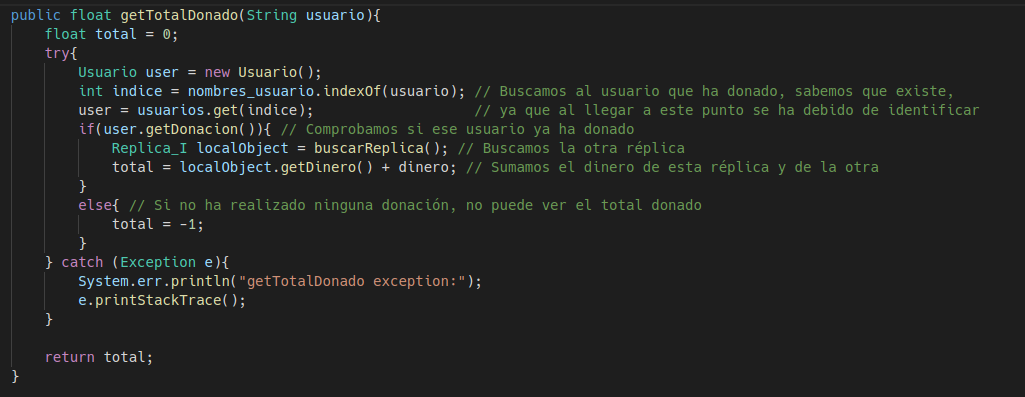
\includegraphics[totalheight=4.9cm]{img/17.png}
		\end{figure}
	\end{enumerate}
	\section{Ejemplo de ejecución}
	Lanzamos la réplica 1:
	\begin{figure}[H]
		\centering
		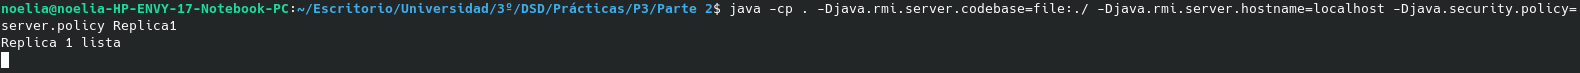
\includegraphics[totalheight=0.58cm]{img/18.png}
	\end{figure}
	Y la réplica 2:
	\begin{figure}[H]
		\centering
		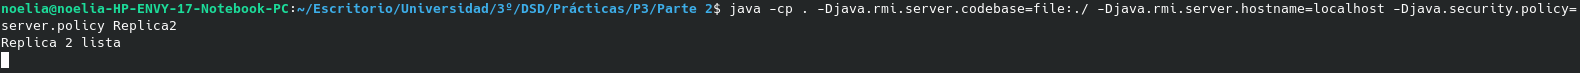
\includegraphics[totalheight=0.58cm]{img/19.png}
	\end{figure}
	Lanzamos el cliente y nos registramos:
	\begin{figure}[H]
		\centering
		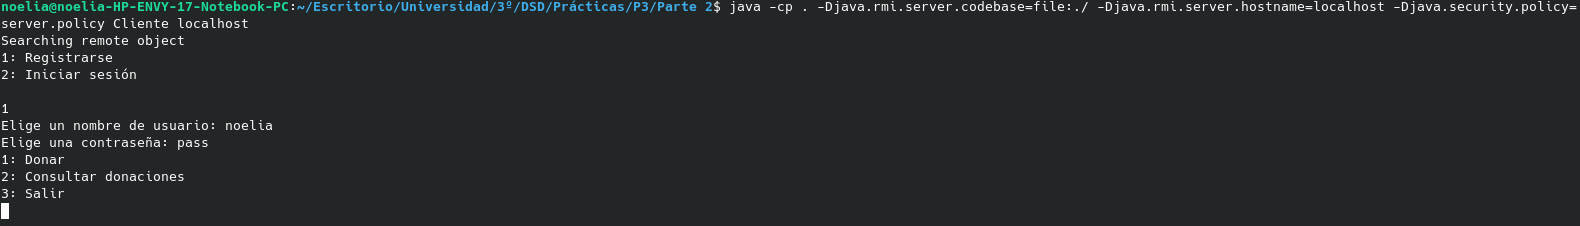
\includegraphics[totalheight=1.8cm]{img/20.png}
	\end{figure}
	La réplica 2 nos avisa de que se han registrado en ella:
	\begin{figure}[H]
		\centering
		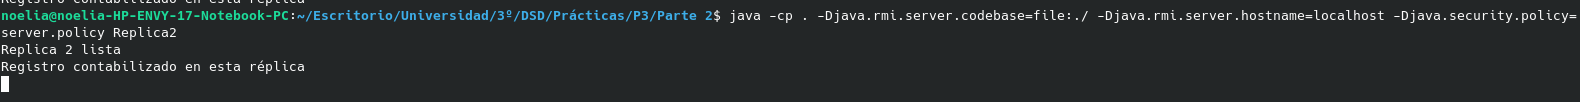
\includegraphics[totalheight=0.82cm]{img/21.png}
	\end{figure}
	Si ahora intentamos registrar otro usuario con el mismo nombre no nos dejará, habrá que elegir otro:
	\begin{figure}[H]
		\centering
		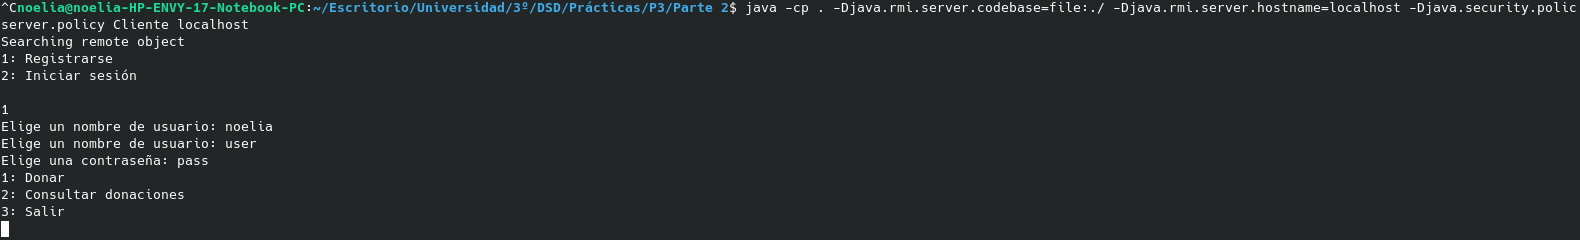
\includegraphics[totalheight=1.95cm]{img/22.png}
	\end{figure}
	Ahora será la réplica 1 la que ha contabilizado el registro:
	\begin{figure}[H]
		\centering
		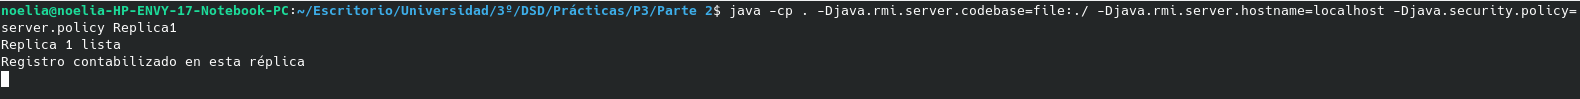
\includegraphics[totalheight=0.81cm]{img/23.png}
	\end{figure}
	Si intentamos iniciar sesión con unos credenciales incorrectos no nos dejará:
	\begin{figure}[H]
		\centering
		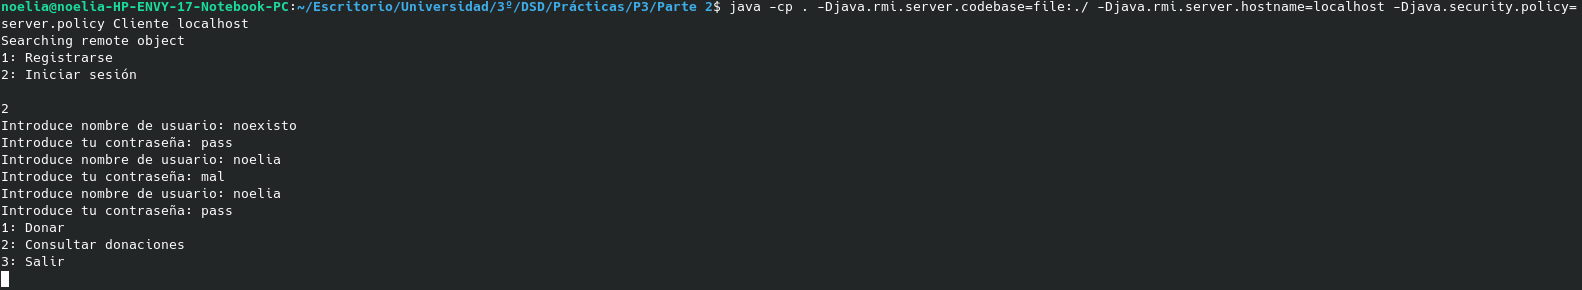
\includegraphics[totalheight=2.36cm]{img/24.png}
	\end{figure}
	Probamos ahora a hacer una donación:
	\begin{figure}[H]
		\centering
		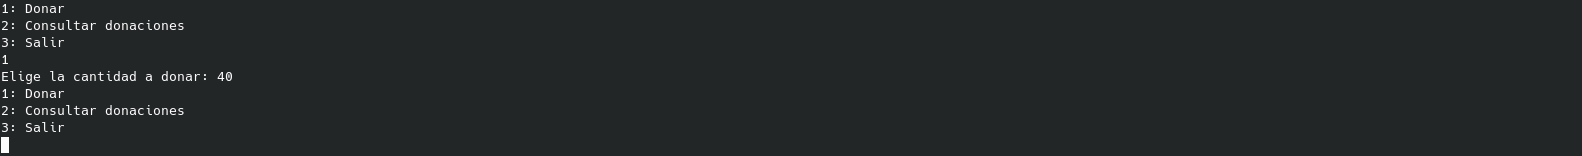
\includegraphics[totalheight=1.27cm]{img/25.png}
	\end{figure}
	La réplica 2 avisa de la donación que ha recibido, ya que es donde está registrado este usuario.
	\begin{figure}[H]
		\centering
		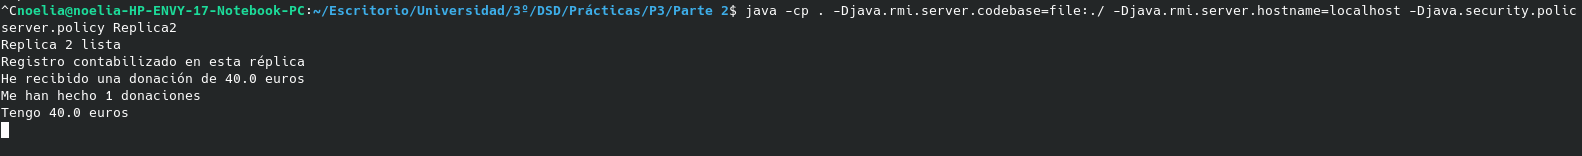
\includegraphics[totalheight=1.27cm]{img/26.png}
	\end{figure}
	Si ahora intentamos consultar el total donado con el otro usuario no nos va a dejar, ya que este usuario no ha hecho ninguna donación:
	\begin{figure}[H]
		\centering
		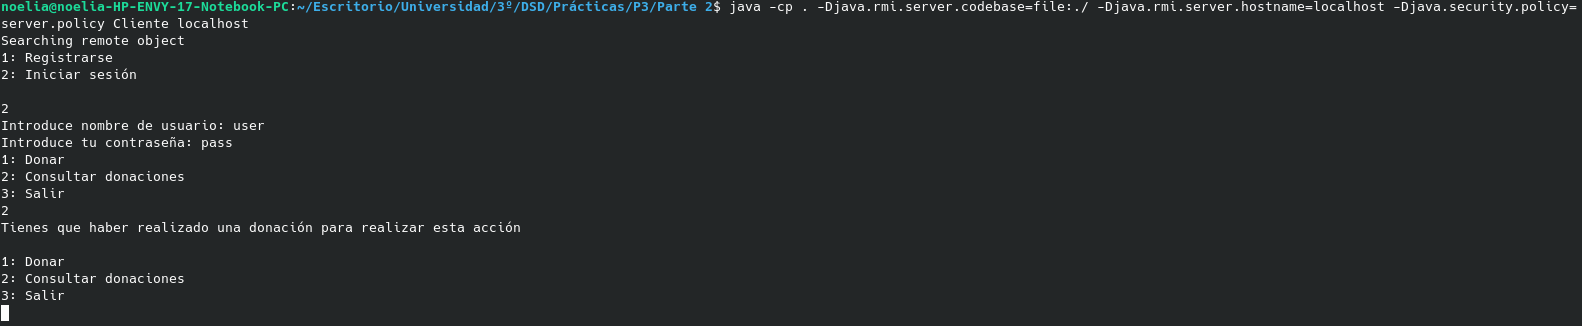
\includegraphics[totalheight=2.6cm]{img/27.png}
	\end{figure}
	Probamos a donar con este usuario:
	\begin{figure}[H]
		\centering
		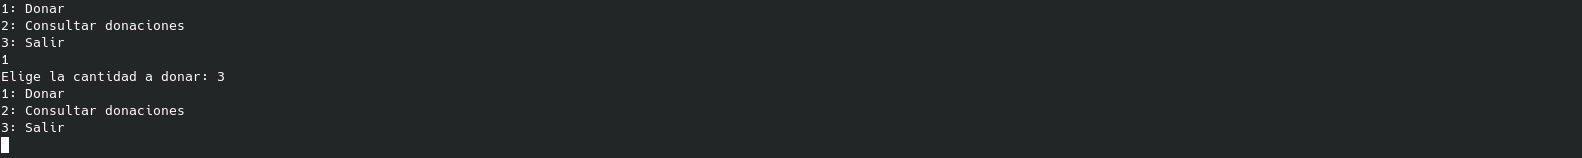
\includegraphics[totalheight=1.27cm]{img/28.png}
	\end{figure}
	Ahora será la réplica 1 la que recogerá la donación:
	\begin{figure}[H]
		\centering
		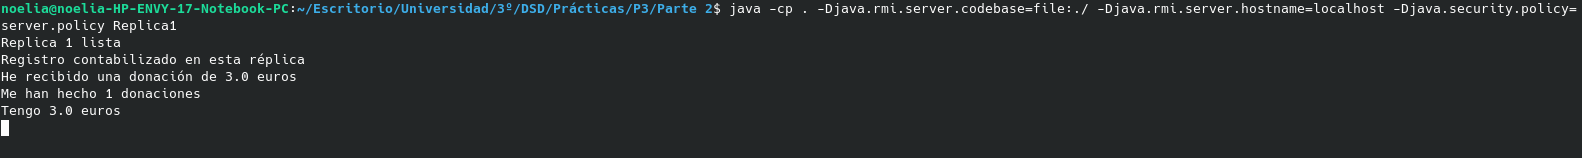
\includegraphics[totalheight=1.27cm]{img/29.png}
	\end{figure}
	Ya sí nos dejará consultar el total donado:
	\begin{figure}[H]
		\centering
		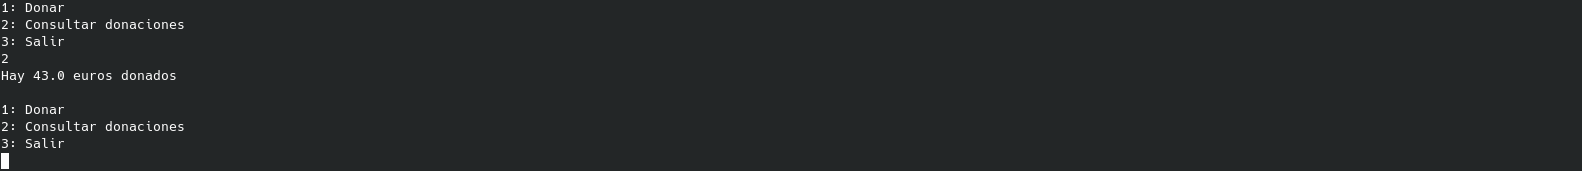
\includegraphics[totalheight=1.37cm]{img/30.png}
	\end{figure}
\end{document}